
\textit{Определение} Когнитивное разивитие

Когнитивное развитие как процесс прохождения стадий, соответствующих развитию интеллектуальных
способностей, описано в работах Жана Пиажет \сite{piaget1952origins}.


\begin{figure}[h]
    \centering
    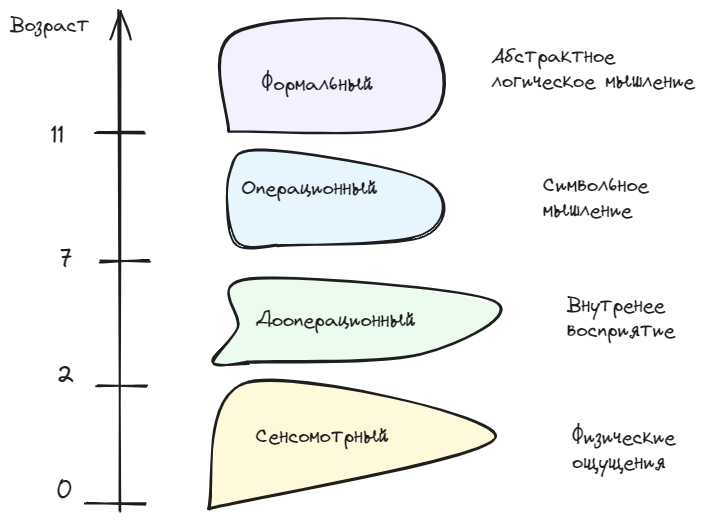
\includegraphics[width=0.5\textwidth]{assets/pedagogic/piage.excalidraw.png}
    \caption{Этапы развития детской психики по Жану Пиаже \сite{piaget1952origins}}
    \label{piage}
\end{figure}

Этапы развития детской психики по Жану Пиаже

\textit{Определение} \textbf{Зона ближайшего развития} — это пространство между тем, что ребёнок уже может сделать самостоятельно, 
и тем, что он может выполнить с помощью более знающего человека.

Концепция, предложенная выдающимся советским психологом Львом Семёновичем Выготским
в его теории социокультуры \cite{выготский2014мышлениеw}. Согласно Выготскому для образования 


\textit{Определение} \textit{Высшие психологические функции}

\begin{figure}[h]
    \centering
    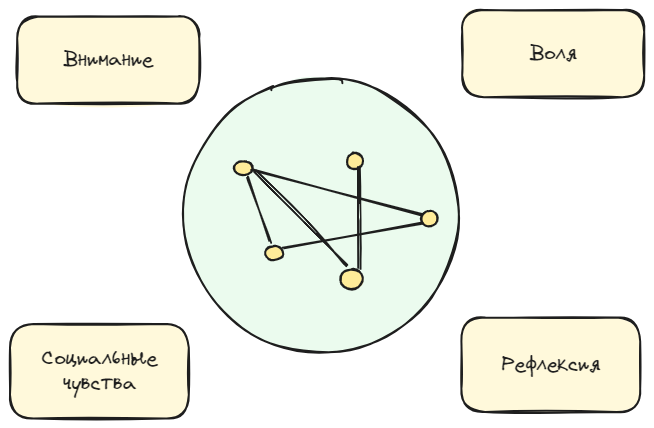
\includegraphics[width=0.5\textwidth]{assets/pedagogic/psy/vpf.excalidraw.png}
    \caption{Результатом высшей психической функции является базовая, воплощаящася в действии}
    \cite{выготский2014мышлениеw}}
    \label{vpf}
\end{figure}










\textit{Определение} \textbf{Поток} — это состояние сознания, характеризующееся полной вовлечённостью и концентрацией
на текущей деятельности, сопровождающееся ощущением контроля, потерей чувства времени и высокой внутренней мотивацией.

Характеристиками потока согласно \cite{csikszentmihalyi2005flow} являются \begin{itemize}
    \item Ясные цели и обратная связь: Деятельность имеет чёткие цели и предоставляет немедленную обратную связь.
    \item Баланс между сложностью задачи и навыками: Задача должна быть достаточно сложной, чтобы бросать вызов, но при этом соответствовать уровню навыков человека, чтобы избегать скуки и тревоги.
    \item Слияние действия и сознания: Человек настолько поглощён деятельностью, что все его действия становятся почти автоматическими и интуитивными.
    \item Потеря самосознания: В потоке человек забывает о себе, своих заботах и тревогах, полностью сосредоточившись на задаче.
    \item Искажение восприятия времени: Время может казаться летящим быстро или, наоборот, замедляться; часы могут пройти как минуты
\end{itemize}

Теория потока задает оптимальную уровень нагрузки согласно навыку \cite{csikszentmihalhi2020finding}. Уровень сложности соответствует

Теория потока активно используется в играх \cite{chen2007flow} и программах непрерывного обучения \cite{jarvis2009routledge}

\textit{Определение} \textbf{Гипотеза о врожденных знаниях} (Innateness hypothesis) - теория в лингвистике и когнитивной науке,
 которая утверждает, что способность к языку является врождённой характеристикой человеческого мозга. 

Гипотеза постулирует наличие:
\begin{itemize}
    \item Врождённого языкового аппарата - врождённой способности,к освоению языка.
    \item Универсальная грамматика - общего набора грамматических принципов и структур, присутствующих во всех языках и врождённых для каждого человека.
    \item Независимости от внешнего опыта: Основные аспекты языковой способности являются врождёнными и не зависят от окружающей среды.
\end{itemize}

Гипотеза имеет статистические подтверждения описанные в работах Ричарда Номски,
использовавшего статистический аппарат синтаксических деревьев для анализа массивного
корпуса естественного языка для  \cite{everaert2015structures}\cite{montague1970universal}.




